\newpage

\subsection{Database-Schema}

\begin{figure}[H]
  \centering
  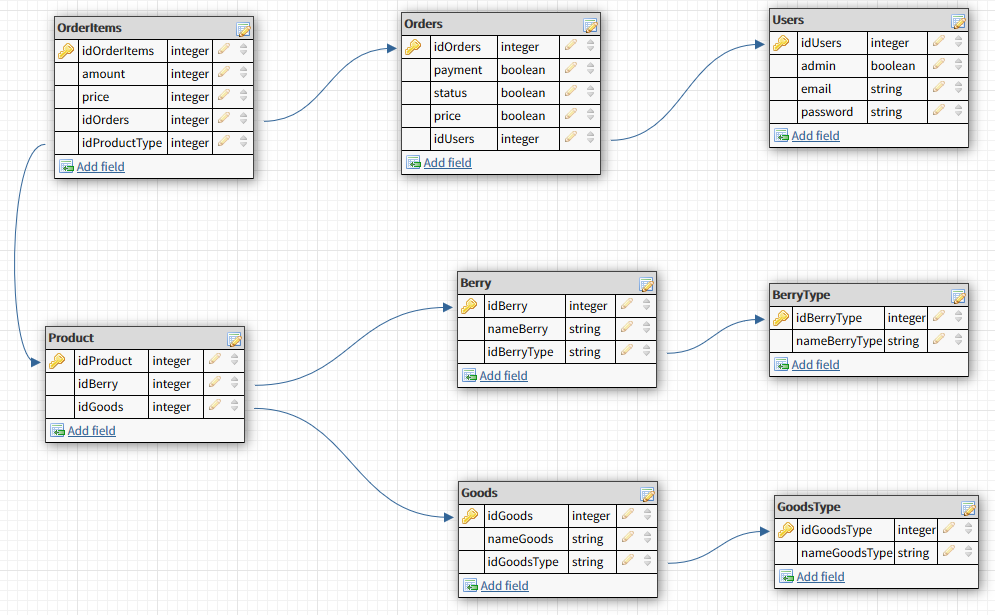
\includegraphics[width=\textwidth]{first_sprint/db_schema.png}
  \caption{\label{fig:schema} The database schema.}
\end{figure}

\textbf{Users:} Keeps the users with an id, email and password. Also a
setting for whether the user is an admin or not.

\begin{itemize}
  \item[\textbf{Orders:}] Keeps orders with a foreign key idUsers to the
    id from table Users. Also keeps whether the order is paid, handled and
    what the price of the order was. The shopping basket is treated as an
    order as well.
  \item[\textbf{OrderItems}] The items of an order with foreign keys
    idOrders and idProduct to the tables Orders and Product.  Keeps the
    amount, price and id of a product in an order.
  \item[\textbf{Product}] Foreign keys idBerry and idGoods to the tables
    Berry and Goods.
  \item[\textbf{Berry}] Foreign key idBerryType to table BerryType. Contains
    name of berry.
  \item[\textbf{Goods}] Foreign key idGoodsType to table GoodsType. Contains
    name of goods.
  \item[\textbf{BerryType}] Contains Berry category.
\end{itemize}
